



% \begin{figure}[H]\centering
% 	\caption{Manhattan Plots of xWAS Results}
%   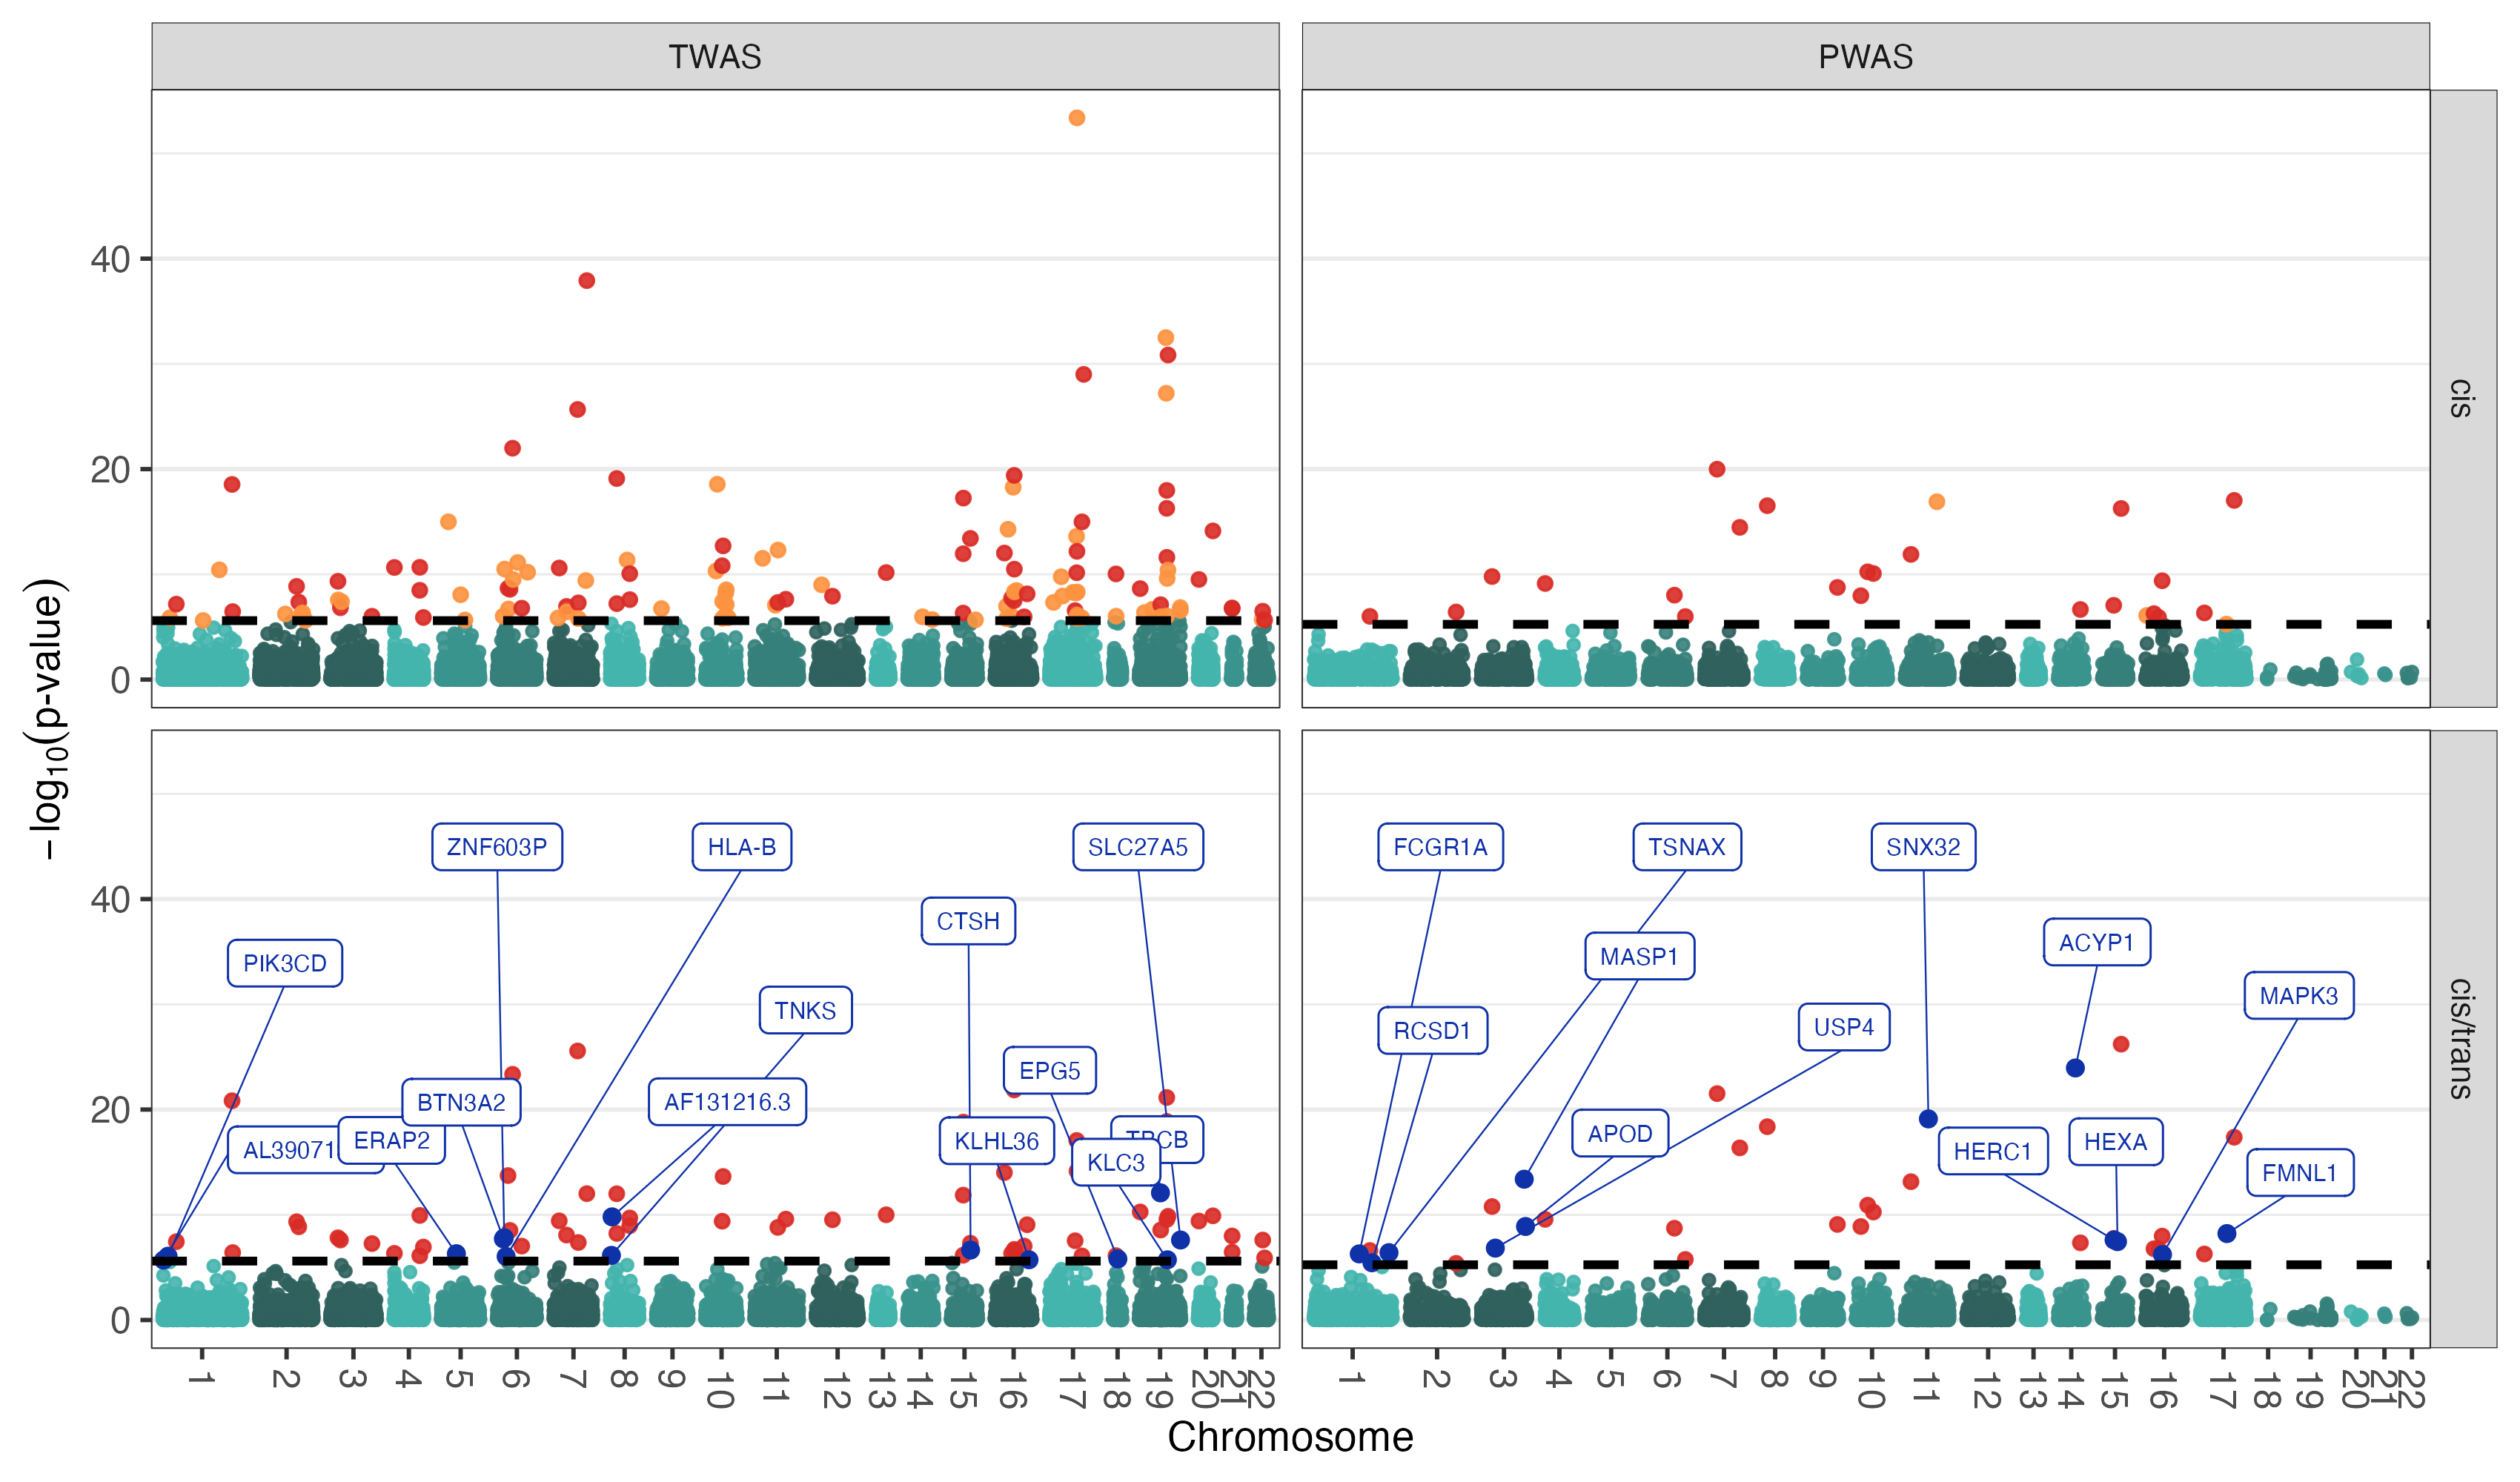
\includegraphics[width=\textwidth]{../figs/manplots_report.png}
%   \label{fig:manplot}
%   {\footnotesize
%   Significant genes identified by only the \textit{cis}/\textit{trans} xWASs are labeled and shown in blue. Significant genes identified by both the \textit{cis}- and \textit{cis}/\textit{trans} models for a given xWAS (TWAS or PWAS) are shown in red. All other significant genes are shown in orange. Non-significant genes are shown in green.}
% \end{figure}



% \begin{figure}[H]\centering
% \caption{Venn Diagrams of Overlapping xWAS Results}
%   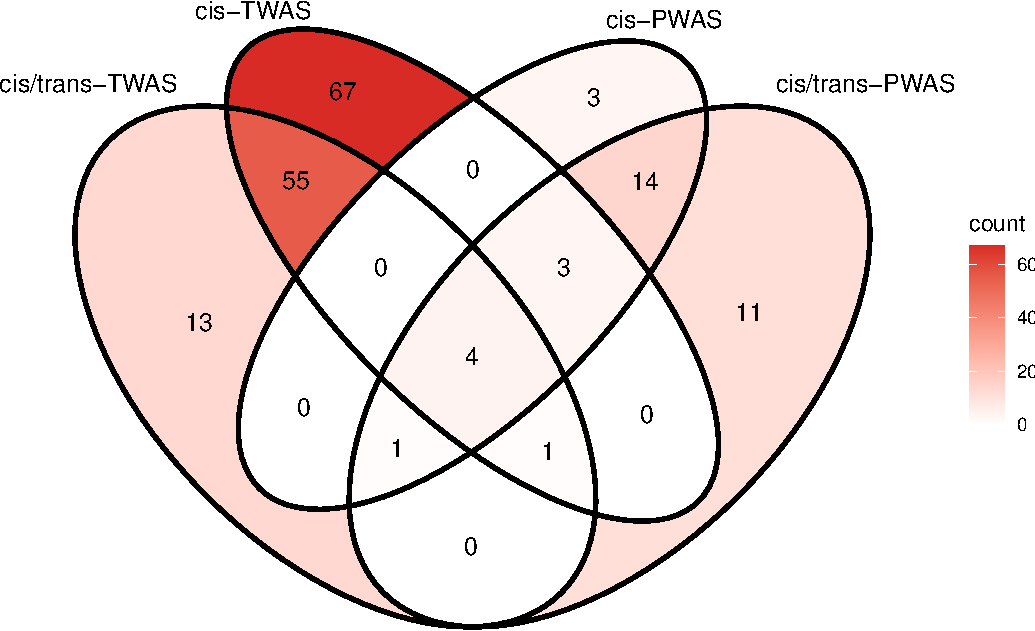
\includegraphics[width=0.8\textwidth]{../figs/venn_report-crop.pdf}
%   \label{fig:venn}
% \end{figure}


\begin{figure}[H]\centering
	\caption{Significant Enriched Paths by pathDIP}
  \includegraphics[width=\textwidth]{../figs/paths_plot.png}
  \label{fig:paths_plot}
\end{figure}


\begin{figure}[H]\centering
	\caption{Venn Diagram of Number of Overlapping Paths for each xWAS}
  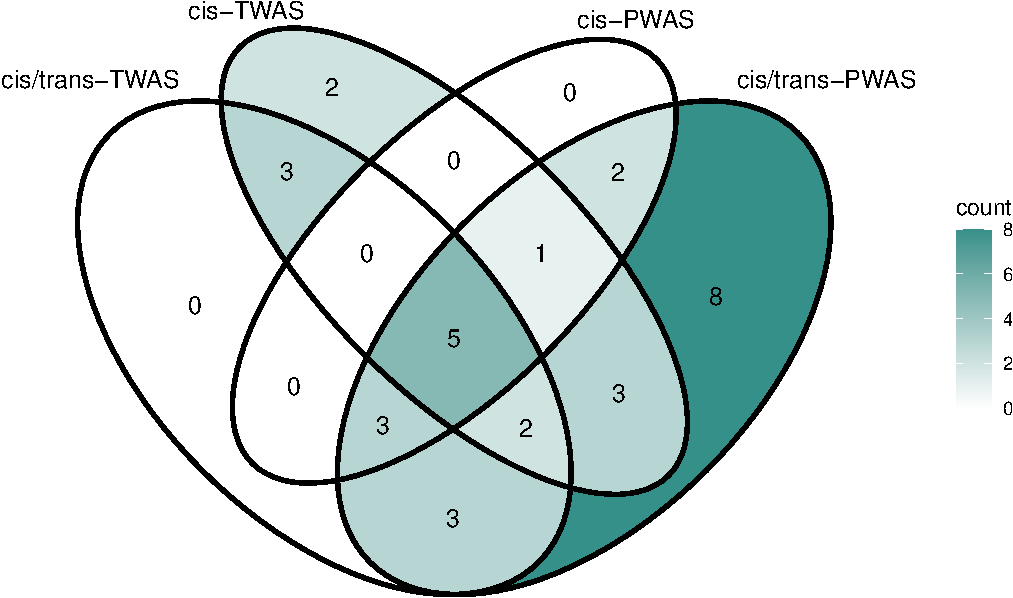
\includegraphics[width=0.8\textwidth]{../figs/paths_venn_report-crop.pdf}
  \label{fig:paths_venn}
\end{figure}

